\documentclass{article}
\usepackage[left=3cm,right=3cm,top=3.5cm,bottom=2cm,
bindingoffset=5mm]{geometry}
\usepackage[utf8]{inputenc}
\usepackage[T1]{fontenc}
% Fuente escalable
\usepackage{lmodern}
\usepackage[english,spanish]{babel}
\usepackage{amsmath}
\usepackage{amssymb,amsfonts,textcomp}
\usepackage{array}
\usepackage{supertabular}
\usepackage{booktabs}
\usepackage{threeparttable}
\usepackage{hhline}
\usepackage[pdftex]{graphicx}
\usepackage{microtype}
% Bibliografia
%\usepackage{bibtex}
\usepackage{biblatex}
%\bibliographystyle{amsplain}
%\bibliography{Bibliografia.bib}
% Formato de unidades
\usepackage{siunitx}
% Graficos
\usepackage{tikz}
% Esquematicos
\usepackage[siunitx, american, cuteinductors, smartlabels]{circuitikz}
% Tablas con ancho establecido por usuario
\usepackage{tabularx}
% Agrega comandos extra al comando tabular
% \toprule, \midrule, \bottomrule
% Multiples figuras dentro de una figura
\usepackage{subfigure}
\usepackage{booktabs}
% Permite unir varias filas en tablas
\usepackage{multirow}
% Encabezados personalizados
\usepackage{fancyhdr}
\usepackage{graphicx}

% Graficas
\usepackage{pgfplots}

% Cabeceras
\pagestyle{fancy}
% Borra cabecera y pie actuales
\fancyhf{}
% Cintillo cabecera
\chead{
	
\includegraphics[width=150mm]{Imagenes/Cabecera.png}
}

\begin{document}
	
	\section{Ruido eléctrico}
		El ruido eléctrico se manifiesta por pequeñas fluctuaciones de corriente y de voltaje en los dispositivos electrónicos. Son múltiples las orígenes o causas del ruido eléctrico, pero todas ellas se pueden agrupar en dos grandes categorías:	
	
		El \emph{ruido extrínseco} es producto de la recepción de señales indeseables generadas en el exterior del dispositivo, y se manifiesta como una perturbación en la repuesta de corriente o voltaje del mismo. Este ruido puede se generado por el hombre cuando tiene su origen en la radiación de artefactos eléctricos o electrónicos. También es producto de fenómenos naturales como lo son relámpagos, tormentas eléctricas, ruido intergaláctico o disturbios atmosféricos en general.
		
		El \emph{ruido intrínseco} es generado el interior del dispositivo, no es producto de la detección de señales externas. Existen diversos tipos de ruido intrínseco mencionados en la literatura, como lo son el \emph{ruido de metralla}, el \emph{ruido de centelleo}, el \emph{ruido ráfaga} y el \emph{ruido térmico}. Este tipo de ruido se debe básicamente al hecho de que la carga eléctrica no es continua, sino que es llevada en cantidades discretas iguales a la carga del electrón.
			
	\subsection{Ruido térmico}
		
		El \emph{ruido térmico} encuentra su origen en el movimiento y colisiones aleatorias de los portadores de carga dentro de los materiales conductores o semiconductores, es uno de los tipos de ruido de mayor importancia en sistemas RF y de microondas. Al ser producto del movimiento térmico de los electrones, guarda relación con la temperatura absoluta T: el ruido térmico es directamente proporcional a T, conforme T se acerque a cero, el ruido térmico también se acercará a cero. Es generado por cualquier elemento de circuito que presente perdidas de energía, como lo son resistores o líneas de transmisión. 
		
		Existen otras fuentes de ruido, externas a un dispositivo, generadas por la absorción atmosférica y la radiación cósmica de fondo, que puede considerarse de origen térmico ya que es producto del movimiento aleatorio de partículas cargadas.
		
	\subsubsection{Voltaje y potencia de ruido}
		
		Todo dispositivo o elemento de circuito que presente perdidas genera ruido térmico. En el caso de un elemento de circuito básico, el resistor, el movimiento aleatorio de los electrones con una energía cinética proporcional a la temperatura se manifiesta como ligeras fluctuaciones de voltaje a través de las terminales del resistor, como se ilustra en la figura \ref{F:RESISTOR_RUIDO}.		
		
		\begin{figure}[h!]			
			\begin{minipage}{0.5\textwidth}		
				\centering	
				\begin{circuitikz}
					\draw 
						(0, 0) to[R, l_=$R$] (0, 2)
						to [short, -o] (2, 2)
						to [open, v^=$v_{N}(t)$] (2, 0)
						to [short, o-] (0, 0);
				\end{circuitikz}
			\end{minipage}	
			\begin{minipage}{0.2\textwidth}	
				\centering					
				\begin{tikzpicture}
					% Esconde marcas de los ejes
					\pgfplotsset{ticks=none} 			
					\begin{axis}[
						black,
						xlabel=$t (\si{\second})$,
						ylabel={$v_N(t) (\si{\volt})$}, 
						domain = 0:10,
						samples = 100,
						xmin = 0, xmax = 10,
						ymin = -1, ymax = 1,
						no markers,
						% Esconde marcas de los ejes
						% yticklabels={,,}
						%,hide axis
						]
						\pgfmathsetseed{1}
						\addplot[color = black] {0.1 * rand }; 										
					\end{axis}
				\end{tikzpicture}	
			\end{minipage}	
			\caption{Fuente de ruido térmico}
			\label{F:RESISTOR_RUIDO}				
		\end{figure}	
		
		No se puede dar una expresión matemática del valor de $v_n(T)$ en forma cerrada: el valor instantáneo de $v_{n}(t)$ no puede ser precisado debido a su naturaleza aleatoria de esta señal.
		
		En su lugar la señal de ruido térmico en un resistor se modela por medio de sus valores estadísticos. El valor medio de la tensión de ruido es cero y su valor cuadrático medio, en un ancho de banda estrecho $B$, viene dado por la aproximación de \emph{Rayleight-Jeans}. Esta puede ser modelado con una fuente de voltaje en serie con un resistor no ruidoso, el equivalente de Thevenin, cuya tensión rms es viene dada por 
		
		\begin{equation}
			V_N = \sqrt{4{\kappa}TBR}
		\end{equation}
		
		\begin{equation}
			\bar{{v_{N}^2}} = 4{\kappa}TBR	
			\label{Ec:VoltajeRuido}	
		\end{equation}
		
		\noindent donde 
		
		\noindent $\kappa = 1.380\cdot10^{-23} \frac{\si{J}}{\si{K}}$ es la constante de Boltzmann.
		
		\noindent $T$ es la temperatura, en grados Kelvin(\si{\K}).
		
		\noindent $B$ es el ancho de banda en \si{\hertz}.
		
		\noindent $R$ es la resistencia, en \si{\ohm}.
		
		De la misma forma, el resistor ruidoso puede modelarse mediante un equivalente de Norton por medio de un resistor no ruidoso en paralelo con una fuente de corriente para modelar la señal de ruido, de valor cuadrático medio
		
		\begin{equation}
			\label{Ec:CorrienteRuido}
			\bar{i_{N}^2} = \frac{4{\kappa}TB}{R}
			\text{$\quad{\kappa}=1.380\dot10^{-23} \, {\si{\joule}}{\si{\kelvin}}$} 	
		\end{equation}
		
		\begin{figure}[h!]
			\begin{minipage}{0.5\textwidth}
				\centering				
				\begin{circuitikz}
					\draw 
					(0, 0) to[R, l_=$R$] (0, 2)
					(0, 4) to [V^=$\bar{i_{N}^2}$] (0, 2) 
					(0, 4) to [short, -o] (2, 4)				
	     		 	(0, 0) to [short, -o] (2, 0);     		 	
	 				
				\end{circuitikz}	
				
				\caption{Modelo de resistor ruidoso}
				\label{Fig:ModeloResistorVoltaje}		
			\end{minipage}
			\quad
			\begin{minipage}{0.5\textwidth}
				\centering				
				\begin{circuitikz}
					\draw 
					(0, 0) to[R, l_=$R$, o-o] (0, 4)
					(0, 1) to [short] (2, 1) 
					(0, 3) to [short] (2, 3)				
					(2, 1) to [I, l=$\bar{v_{N}^2}$] (2, 3);				
				\end{circuitikz}			
				\caption{Modelo de resistor ruidoso}
				\label{Fig:ModeloResistorCorriente}	
			\end{minipage}		
		\end{figure}	
			
		
		\noindent donde $R$ es la resistencia en \si{\ohm}, ${\Delta}f$ es el ancho de banda en \si{\hertz} sobre el cual el ruido es medido. Las expresiones anteriores son validas hasta frecuencias de microondas. El ruido térmico en un resistor es \emph{independiente} de su composición.
		
	\subsubsection{Máxima potencia de ruido disponible}
		
		Los valores de tensión y corriente de los modelos son útiles para fines teóricos. En la practica, es común especificar las características de una señal de ruido por medio de su \emph{potencia de ruido disponible}, la cual se define como la máxima potencia entregada por la fuente de ruido a un resistor de carga. Se sabe que la máxima potencia que puede entregar un generador con impedancia interna $Z_S$ ocurre cuando se la impedancia de carga es igual al complejo conjugado del generador, $Z_L = Z_S$
		
		\begin{figure}[h!]
			\centering		
			\begin{circuitikz}
			\draw
				(4, 0) rectangle ++(2, 2)
				(5, 1) node[below] {Ancho de banda B}	
				(6, 1.8) to[short, -o] 
				(7, 1.8) to[short] (8, 1.8)
				to[R, l^=$R$] (8, 0.2)
				to[short] (7, 0.2)
				to[short, o-] (6, 0.2)
				(0, 1.8) to[V, l=$V_n$] (0, 0.2)
				(0, 1.8) to[R = $R$, -o] (2, 1.8) 
				to[short] (4, 1.8) 
				(0, 0.2) to[short, -o] (2, 0.2)
				to[short] (4, 0.2);				
			\end{circuitikz}
			\caption{Máxima transferencia de potencia desde un resistor ruidoso a una carga sobre un ancho de banda B.}
			\label{Fig:MaximaTransferenciaPotencia}
		\end{figure}		
	
		Así pues, la máxima potencia de ruido disponible puede ser calculada como
		
		\begin{equation}
			P_n = \left(\frac{V_N}{2}\right)^2\frac{1}{R} = \frac{V_n^2}{4R} = {\kappa}TB
			\label{Ec:PotenciaRuidoDisponible}
		\end{equation}		
		
		\noindent donde $V_N$ es el voltaje de ruido rms del resistor. De la ecuación \eqref{Ec:PotenciaRuidoDisponible} se infiere que
		
		\begin{itemize}
			\item La potencia de ruido se decrementa en la medida que el ancho de banda del sistema se decrementa.
			\item Los sistemas con ancho de banda pequeños colectan menos ruido.
			\item La potencia de ruido disminuye a medida que la temperatura desciende. 
			\item La potencia de ruido depende del ancho de banda absoluto, pero no de la frecuencia central de la banda.
						
		\end{itemize}
	
		Como el ruido térmico resulta independiente de la frecuencia, se le conoce como \emph{ruido blanco}, en analogía a la luz blanca la cual esta compuesta de múltiples frecuencias de luz visible. Experimentalmente y verificado por la mecánica cuántica, el ruido térmico es independiente de la frecuencia para $0 < f < 1000\si{\giga\hertz}$.
		
	\subsubsection{Densidad espectral}
		
		La potencia de ruido de la ecuación \eqref{Ec:PotenciaRuidoDisponible} puede ser representada en términos de la densidad espectral. Como la ecuación \eqref{Ec:PotenciaRuidoDisponible} es independiente de la frecuencia, la densidad espectral también ser independiente de la frecuencia, esta viene dada por
		
		La potencia de ruido por unidad de ancho de banda $S$ que un resistor en equilibrio térmico a una una temperatura T entrega a través de sus terminales viene dada por. La densidad de potencia de ruido para el modelo Thevenin del resistor viene dada por
				
		\begin{equation}
			S_N(\omega) = \frac{P_N}{2B} = \frac{{\kappa}T}{2} = \frac{{\eta}_0}{2}
		\end{equation}	
		
		\noindent donde se ha tomado $\frac{{\eta}_0}{2} = \frac{{\kappa}T}{2}$. Esta última ecuación es conocida como la \emph{potencia de ruido bilateral} para el ruido blanco, el factor $1/2$ es para tomar en cuenta el ancho de banda de $-B$ a $B$ (\si{\Hz})
		
	\subsubsection{Temperatura de ruido equivalente}
		
		Para una fuente de ruido blanca como la densidad espectral de ruido no depende de la frecuencia (al menos en el rango de frecuencia de interés), puede ser modelada por una \emph{fuente equivalente de ruido térmico} la cual se caracteriza por una \emph{temperatura de ruido equivalente}. En la figura \ref{Fig:FuenteRuidoBlanco} una fuente arbitraria de ruido blanco con impedancia interna $R$ alimenta una impedancia de carga R con una potencia de ruido $N_O$. La fuente de ruido puede ser reemplazada por un resistor ruidoso de valor R a una temperatura $T_e$, la cual es la temperatura a la cual debe someterse el resistor $R$ para que entregue una densidad de potencia espectral igual a $N_0$. Se tiene entonces que 
		
		\begin{equation}
			N_O = {\kappa}BT_e
			\label{Ec:DensidadPotenciaEspectral2}
		\end{equation}
		
		\begin{equation}
			T_e = \frac{N_O}{{\kappa}B}
			\label{Ec:TemperaturaEquivalenteRuido}
		\end{equation}	
		
		
		\begin{figure}[h!]
			\centering
			\begin{circuitikz}
				\draw
				(0, 0) rectangle ++(2, 2)
				(1, 1) node[below] {Fuente de ruido blanco}	
				(2, 1.8) to[short, -o] (3, 1.8)
				to[short,  i=$N_{O}$] (4, 1.8)
				to[R, l^=$R$] (4, 0.2)
				to[short] (3, 0.2)
				to[short, o-] (2, 0.2);
 
			\end{circuitikz}	
			\qquad
			\begin{circuitikz}	
				\draw[dotted]
				(0, 0) rectangle ++(2, 2);	
				\draw
				(1, 0.2) to[R, l_=$R$] (1, 1.8)
				to[short, -o] (3, 1.8)
				to[short,  i=$N_{O}$] (4, 1.8)
				to[R, l^=$R(T_E)$] (4, 0.2)
				to[short, -o] (3, 0.2)
				to[short] (1, 0.2);
			\end{circuitikz}	
			\caption{Red ruidosa remplazada por resistor a temperatura equivalente}
			\label{Fig:RED_SIN_RUIDO}
		\end{figure}		
	
	\subsubsection{Figura de ruido}
	
	La \emph{figura de ruido} permite medir la degradación de la relación señal a ruido entre la entrad y salida de un componente. De la misma forma que la temperatura de ruido equivalente, permite caracterizar un dispositivo de RF o de microondas. La figura de ruido como figura de merito indica que tan eficaz es un dispositivo para discriminar señales en presencia de ruido, el cual puede ser externo o generado por el propio dispositivo en cuestión.
	
	La figura de ruido es definida como
	
	\begin{equation}
		F = \frac{Relación señal ruido entrada}{Relación señal ruido salida} = \frac{\frac{S_i}{N_i}}{\frac{S_o}{N_o}}
		\label{Ec:FiguraRuido1}
	\end{equation}
	
	\noindent donde $S_i$ y $N_i$ son la potencia de señal y ruido a la entrada del dispositivo respectivamente, $S_o$ y $N_o$ son la potencia de señal y ruido a la salida del dispositivo. La definición de figura de ruido exige que la potencia de ruido a la entrada provenga de un carga acoplada a una temperatura de TO = 290 K.
	
	\begin{figure}[h!]
		\centering		
		\begin{circuitikz}
			\draw
			(0, 3) to [V, l=$S_i$] (0, 0.5) 
			(0, 3) to[R=$R$] (2, 3)
			(0, 0.5) to[short, i=$ $] (2, 0.5)
			(2, 0) rectangle ++(3, 3.5)
			(5, 3)to[short] (7, 3)
			to[R=$R$] (7, 0.5)
			(5, 0.5) to[short, i = $ $] (7, 0.5)
			(4, 2) node[below] {Red ruidosa $G, B, T_e$};			
		\end{circuitikz}
		\caption{Máxima transferencia de potencia desde un resistor ruidoso a una carga sobre un ancho de banda B.}
		\label{Fig:SistemaFiguraRuido}
	\end{figure}		
	
	En la figura \ref{Fig:SistemaFiguraRuido} una red ruidosa caracterizada por una ganancia $G$, que posee un ancho de banda $B$ y una temperatura equivalente de ruido $T_e$, es alimentada con una señal de potencia $S_i$ y una señal de ruido $N_i$. Este ruido es modelado por un resistor de fuente $R$, el cual debe estar encontrarse a una temperatura $T_0 = 290\si{\kelvin}$ para cumplir con la definición de figura de ruido. La potencia de ruido en la entrada de la red es entonces
	
	\begin{equation}
		N_i = {\kappa}T_0B
		\label{Ec:RuidoEntrada}
	\end{equation}	
	
	La potencia de señal a la salida de la red resulta
	
	\begin{equation}
		S_o = GS_i
		\label{Ec:SeñalSalida}
	\end{equation}		
	
	La señal de ruido presente en la salida de la red se debe tanto a la señal de ruido en su entrada $N_i$ y al ruido intrínseco que genera la propia red en su interior y lo agrega en la salida. Si se define este ruido como $N_a$, la potencia de ruido total a la salida para esta red es la suma del ruido amplificado a la entrada y del ruido generado internamente por la propia red	

	\begin{equation}
		N_o = GN_i + N_a
		\label{Ec:RuidoSalida}
	\end{equation}		
	
	La figura de ruido para la red de la figura \ref{Fig:SistemaFiguraRuido} 
	
	\begin{equation}
		F = \frac{\frac{S_i}{N_i}}{\frac{S_o}{N_o}} = \frac{\frac{S_i}{N_i}}{\frac{GS_i}{GN_i+N_a}} = \frac{(GN_i+N_a)S_i}{GS_iN_i}
		\label{Ec:FiguraRuido2}
	\end{equation}		
	
	Simplificando se obtiene
	
	\begin{equation}
		F = 1  + \frac{N_A}{GN_i}
		\label{Ec:FiguraRuido3}
	\end{equation}			
	
	De la ecuación anterior, para una red determinada con $N_a$ fijo, el valor de F dependerá del valor de $N_i$. Debido a que $N_a$ no depende de ni guarda correlación $N_i$, se debe fijar $N_i$ como valor de referencia en base a un estándar (IEEE).		
	
	La cantidad $\frac{N_a}{G}$ dentro de la ecuación \eqref{Ec:FiguraRuido3} puede considerarse como el ruido generado por la propia red referido a su entrada. 
	
	Para la red de la figura \ref{Fig:SistemaFiguraRuido} se puede reescribir la ecuación \eqref{Ec:FiguraRuido1} en función de la temperatura equivalente de ruido de la red. El ruido generado por esta en función de $T_e$ es $N_i = {\kappa}BT_e$ y esta referido a su entrada. Sustituyendo este valor en la ecuación \eqref{Ec:FiguraRuido1}
	
	\begin{equation}
		F = \frac{\frac{S_i}{{\kappa}T_0B}}{\frac{GS_i}{{\kappa}GB(T_0 + T_e)}}=\frac{S_i}{GS_i}\frac{{\kappa}GB(T_0 + T_e)}{{\kappa}T_0B}
	\end{equation}
	
	Simplificando resulta
	
	\begin{equation}
		F = 1 + \frac{T_e}{T_0}
		\label{Ec:FiguraRuido4}
	\end{equation}	
	
	\subsubsection{Razón de ruido en exceso y fuentes de ruido}
	
	Una forma directa para medir la temperatura equivalente de ruido es alimentar el dispositivo con una fuente de ruido con valores de potencia conocidos y medir el incremento de la potencia de ruido a la salida. Debido a que la potencia de ruido generada por un resistor es muy pequeña, existen fuentes de ruido activas para este propósito. Las fuentes de ruido activas están basadas en tubos de vacío o diodos semiconductores.
	
	Los generadores de ruido activos pueden ser caracterizados a través de la temperatura equivalente, pero  una medida común de la potencia de ruido de esto dispositivos es la razón de ruido en exceso
	
	\begin{equation}
		ENR = \frac{N_G-N_0}{N_0} = \frac{T_G - T_0}{T_0}
	\end{equation}
	
	\begin{equation}
		ENR(\si{\decibel}) = 10\log(ENR)
	\end{equation}	
	
	\noindent donde $N_G$ y $T_E$ son la potencia de ruido y la temperatura equivalente del generador de ruido, y $N_O = {\kappa}T_0B$ con $T_0 = 290\si{\kelvin}$ son la potencia de ruido y la temperatura asociada a una fuente pasiva (considerando una carga acoplada) a temperatura ambiente.
	
	\subsubsection{Medición de figura de ruido. El factor Y.}	
	
	Cuando a un dispositivo lineal de dos puertos se alimenta con una fuente de ruido térmico a una temperatura TS como se indica en la figura \ref{Fig:RuidoRed2Puertos}, la potencia  medida a su salida puede representarse como	
	
	\begin{equation}
		N_o = {\kappa}GBT_s + N_a 
	\end{equation}
	
	\noindent En donde $N_a$ representa el ruido interno generado por el propio dispositivo y el término ${\kappa}GBT_s$ representa el ruido térmico de la fuente a la salida. Esta ecuación representa la ecuación de una recta, donde la potencia de salida depende de manera lineal de la temperatura de la fuente $T_s$.
	
	\begin{figure}[h!]
		\begin{minipage}{0.5\textwidth}
			\centering
			\begin{circuitikz}
				\ctikzset{bipoles/amp/width=1.2}
				\draw
				(0, 0) to [R=$R$] (0, 3) 				
				to[amp, t=$DUT$, -o] (4, 3)		
				(0,0) node[ground]{};										
				\draw 
				(1.2, 1.5) node[below] {$T_s$}	
				(1.2, 1.0) node[below] {$N_{s}={\kappa}T_S$}
				(4.0, 3.0) node[below] {$N_{o}={\kappa}GBT_S$};
			\end{circuitikz}			
		\end{minipage}
		\begin{minipage}{0.5\textwidth}
			\centering
			\begin{tikzpicture}
				% Esconde marcas de los ejes
				\pgfplotsset{ticks=none} 			
				\begin{axis}[
					black,
					xlabel=$T_S (\si{\kelvin})$,
					ylabel={$N_o (\si{\watt}/\si{\hertz})$}, 
					domain = 0:10,
					samples = 100,
					xmin = 0, xmax = 10,
					ymin = 0, ymax = 10,
					no markers,
					% Esconde marcas de los ejes
					% yticklabels={,,}
					%,hide axis
					]
					\pgfmathsetseed{1}
					\addplot[color = black] {2 + 6 * x / 10}; 		
					\addplot[color = black, domain = 3:6, dotted] {3.8}; 		
					\addplot[color = black, dotted] coordinates {(3, 0) (3, 3.8)};	
					\addplot[color = black, dotted] coordinates {(6, 0) (6, 5.6)};										
					\node at (axis cs:1, 2) [anchor=north east] {$N_A$};		
					\node at (axis cs:6, 3.8) [anchor=north east] {$G = {\kappa}RT_SB$};		
					\node at (axis cs:3, 1.0) [anchor=north east] {$T_C$};		
					\node at (axis cs:6, 1.0) [anchor=north east] {$T_H$};									
				\end{axis}
			\end{tikzpicture}
		\end{minipage}
		\caption{Respuesta al ruido DUT}
		\label{Fig:RuidoRed2Puertos}
	\end{figure}		
	
	La mayoría de los dispositivos de RF y microondas generan muy bajos niveles de ruido, resulta difícil aplicar el método de medición directa de esta potencia de ruido de manera precisa. En cambio, una técnica que vence esta dificultad utilizando una razón de medidas de potencia  es llamada el factor Y.  La técnica se resume en la figura , en donde un dispositivo bajo prueba -el DUT- se alimenta desde una de dos fuentes de ruido acopladas a distintas temperaturas.
	
	Para medir la figura de ruido empleando el factor Y, se conecta a la entrada del dispositivo objeto de estudio, un generador de ruido, el cual puede ser un diodo con polarización inversa. La temperatura de ruido equivalente guarda relación con con la corriente de polarización inversa del diodo, esta corriente se hace variar en dos niveles, \emph{encendido (ON)} y \emph{apagado (OFF)}, lo que equivale a aplicar una fuente de ruido con dos temperaturas equivalentes de ruido, la temperatura fría ($T_C$) y la temperatura caliente ($T_H$). Para las temperatura de fuente $T_C$, se registrará en la salida del dispositivo la potencia N1; para la temperatura caliente se registrará una temperatura caliente $T_H$:	
	
	\begin{equation}
		\begin{align}
			N_1 &= N_a+{\kappa}GBT_C \\
			N_2 &= N_a+{\kappa}GBT_H 
		\end{align}		
	\end{equation}
	
	Ya que el ruido generado por las fuentes no esta correlacionado con el ruido generado por el DUT, el ruido es aditivo y el ruido total a la salida del DUT es la suma de la potencia de ruido de la fuente y la potencia de ruido generada por el propio DUT.
		
	La razón de ruido en exceso (ENR) para la fuente utilizada puede expresarse en función de las temperaturas $T_C$, $T_H$ y la temperatura de referencia $T_0$
	
	\begin{equation}
		ENR = \frac{T_H - T_C}{T_0}
		\label{Ec:EnrFactorY}
	\end{equation}
	
	El \emph{factor Y} se define como	
	
	\begin{equation} 
		Y = \frac{N_2}{N_1} = \frac{N_a+{\kappa}GBT_C}{N_a+{\kappa}GBT_H}
	\end{equation}
	
	De esta ecuación se puede resolver para encontrar la potencia de ruido generada por el dispositivo.
	
	\begin{equation}
		N_a = \frac{{\kappa}GB(T_H - T_C) + (1 - Y)T_C}{Y - 1}
	\end{equation}
	
	Al emplear la expresión para ENR de la ecuación \eqref{Ec:EnrFactorY}
	
	\begin{equation} 
		N_a = {\kappa}GB\left(\frac{T_0ENR}{Y-1}-T_C\right)
	\end{equation}
	
	El factor Y puede ser expresado en función de la temperatura equivalente de ruido $T_e$ del dispositivo, resulta
	
	\begin{equation} 
		Y = \frac{N_2}{N_1} = \frac{{\kappa}GB(T_H + T_e)}{{\kappa}GB(T_C + T_e)}		
	\end{equation}	
	
	Aplicando en esta última ecuación la expresión para ENR de la ecuación \eqref{Ec:EnrFactorY}, se resuelve $T_e$
	
	\begin{equation} 
		T_e = \frac{T_0ENR}{Y - 1} - T_C
	\end{equation}
	
	\subsubsection{Medición de figura de ruido dispositivos en cascada.}
			
		\begin{figure}[h!]
			\centering
			\begin{circuitikz}
				\draw 
				(0, 0) to[R, l=${\kappa}T_o$] (0, 4)
				(0, 4) to[short, -o] (1, 4)
				(1, 4) to[amp, t=$A_{1}$] (4, 4)
				(4, 4) to[amp, t=$A_{2}$] (7, 4)
				(7, 4) to[amp, t=$A_{3}$, -o] (10, 4)
				(10, 4) to[short] (12, 4)
				(12, 4) to[R, l=$R_{L}$] (12, 0)
				(12, 0) to[short] (11, 0)
				(11, 0) to[short, o-o] (1, 0)
				(1, 0) to[short] (0, 0)
				node[ground] {};
				
				\draw
				(2.5, 4.5) node[above] {$N_{A1}, G_{1}, B$}
				(5.5, 4.5) node[above] {$N_{A2}, G_{2}, B$}
				(8.5, 4.5) node[above] {$N_{A3}, G_{3}, B$};
				
				\draw
				(1, 2.8) node[below] {${\kappa}T_{O}B$}
				
				(4, 2.8) node[below] {${\kappa}T_{O}BG_{1}$}
				(4, 2.3) node[below] {$N_{A1}$}
				
				(7, 2.8) node[below] {${\kappa}T_{O}BG_{1}G_{2}$}
				(7, 2.3) node[below] {$BG_{2}N_{A1}$}
				(7, 1.8) node[below] {$N_{A2}$}
				
				(10, 2.8) node[below] {${\kappa}T_{O}BG_1{1}G_{2}G_{3}$}
				(10, 2.3) node[below] {$BG_{2}G_{3}N_{A1}$}
				(10, 1.8) node[below] {$BG_{3}N_{A2}$}
				(10, 1.3) node[below] {$N_{A3}$};
				
			\end{circuitikz}
			\caption{Dispositivos en cascada}\label{Fig:AmplificadoresCascada} 
	\end{figure}

	\begin{align}
		N_o &= {\kappa}T_0BG_1G_2G_3 + G_2G_3N_{A1} + G_3N_{A2}+N_{A3} \\
		N_o &= {\kappa}ToBG_1G_2G_3(1 + \frac{N_{A1}}{{\kappa}BG_1T_0}  + \frac{N_{A2}}{{\kappa}BG_1G_2T_0}+\frac{N_{A3}}{{\kappa}T_0BG_1G_2G_3}) \\	
		N_o &= {\kappa}ToBG_1G_2G_3(F_1 + \frac{F_2 - 1}{G_1} + \frac{F_3 - 1}{G1G2})
	\end{align}
	
	Como la figura de ruido de los dispositivos en cascada viene dada por
	
	\begin{align} 
		F &= \frac{\text{Ruido total a la salida}}{\text{Ruido de $R_s$ en la salida}} \\
		F &= \frac{N_o}{{\kappa}T_0BG_1G_2G_3} \\
		F &= F_1 + \frac{F_2 - 1}{G_1} + \frac{F_3 - 1}{G_1G_2}		
	\end{align} 		
	
	\subsubsection{Medición de figura de ruido empleando el factor Y.}	
	
	\begin{figure}[h!]
		\centering
		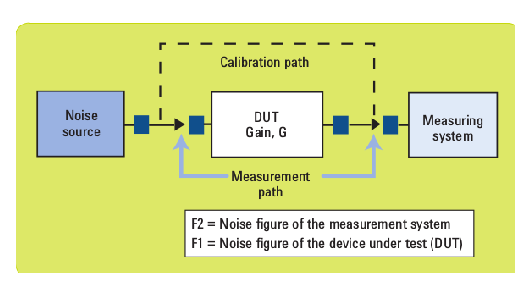
\includegraphics[width=10cm]{Imagenes/InstrumentacionFactorY.pdf}
		\caption{Montaje para medición de figura de ruido con el factor Y}
	\end{figure}

	\begin{figure}[h!]
		\centering
		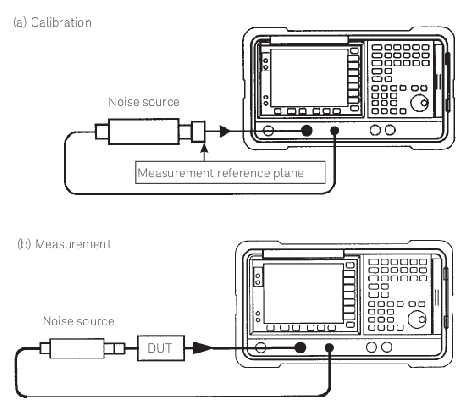
\includegraphics[width=16cm]{Imagenes/InstrumentacionCalibracionMedicion.pdf}
	\end{figure}

	\begin{figure}[h!]
		\centering
		\begin{circuitikz}
			\ctikzset{bipoles/amp/width=1.2}
			\draw 
			(0, 0) to[R, l=$2{\kappa}T_{S}B\si{\watt}$] (0, 3)
			to[short, -o] (1,3)
			to[amp, t=$DUT$, -o] (3, 3)				
			to[short, l=$Z_{0}$, -o] (4, 3)
			to[R, l=$R$] (4, 0)
			to[short] (3, 0)
			to[short, o-o] (1, 0)
			to[short] (0, 0)
			node[ground] {};				
			\draw 
			(2.5, 1.8) node[below] {${\kappa}T_{S}B$}	
			(6.5, 1.5) node[below] {$N_{O}$};
		\end{circuitikz}
		\caption{Respuesta al ruido DUT}\label{Fig:RespuestaRuidoDut} 
	\end{figure}

\end{document}